{\bf System Design} : Systems design is the process or art of defining 
the architecture, components, modules, interfaces, and data for a 
system to satisfy specified requirements. One could see it as the 
application of systems theory to product development. There is some 
overlap with the disciplines of systems analysis, systems architecture 
and systems engineering.
\begin{enumerate}
\item  External design: External design consists of conceiving, 
planning out and specifying the externally observable characteristics 
of the software product. These characteristics include user displays or 
user interface forms and the report formats, external data sources and 
the functional characteristics, performance requirements etc. External 
design begins during the analysis phase
and continues into the design phase.
\item  Logical design: The logical design of a system pertains to an 
abstract representation of the data flows, inputs and outputs of the 
system. This is often conducted via modeling, which involves a 
simplistic (and sometimes graphical) representation of an actual system. 
In the context of systems design, modelling can undertake the following 
forms, including:
\begin{itemize}
\item Data flow diagrams
\item Entity Relationship Diagrams
\end{itemize}
\item  Physical design: The physical design relates to the actual input 
and output processes of the system. This is laid down in terms of how 
data is input into a system, how it is verified/authenticated, how it 
is processed, and how it is displayed as output.
\end{enumerate}


\newpage
\begin{figure}[h]
\centering 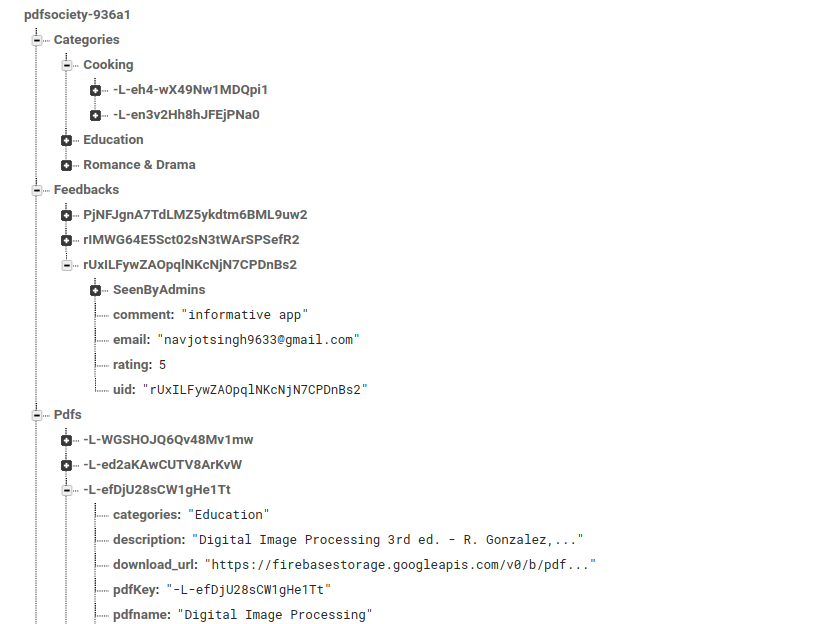
\includegraphics[scale=0.5]{images/db1.png}

\end{figure}
\newpage
\begin{figure}[h]
\centering 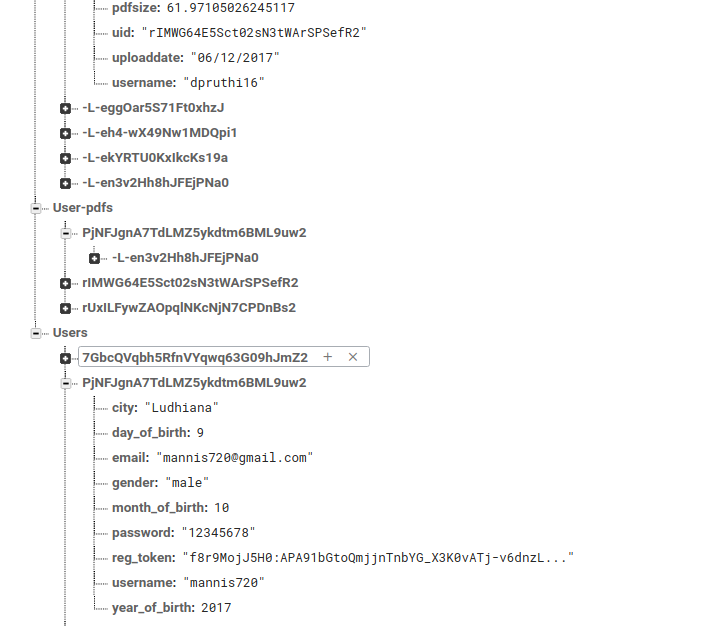
\includegraphics[scale=0.5]{images/db2.png}
\caption{Database Design}
\end{figure}
